
\chapter{Some Notes on Mathematical Modeling}
These are the steps for mathematical modeling that I have gathered by thinking deep and observing what is happening around me. How my supervisors attack a problem, what is the thought process of professor X in dealing with a problem at one glance, what are the concerns about a specific type of problem (like Stock's problem in PDE theory which is a saddle-node type problem), and what are the main tools to address that problem. These steps in modeling a phenomena mathematically gives me a sense of orientation in a busy world full of new things. This section will be developed overtime, and at some point it can be a chapter of my thesis.

\begin{summary}
	The primary purpose of these notes is to locate the stage of any ongoing project. Also, I will do my best to prepare a kind of checklist for each step that can be used to evaluate the progress of the sub-steps of the project.
\end{summary}

\section{STEP 0: Understanding the phenomena we want to study}

\section{STEP I: Converting Natural Phenomena to a Mathematical Problem }
This step is one of the steps that looks very strange for me. Early from calculus courses and elementary ODE, PDE courses, we can see phrase like ``this Dirichlet boundary condition along with an elliptic PDE models a rod that its two ends are covered with ice at temperature 0'', or ``This saddle-point problem named Stokes problem models a non-compressible fluid''. But they never talk about why this is true, and even how this is possible? Why a bunch of numbers and functions should mimic a very complex phenomena?

There are some very interesting papers written to explain why the mathematics is so effective in modeling the natural world (see \autoref{fig:mathmodelingmatheffectiveness}). In my opinion, this step, although innocent looking, is a totally non-trivial step. Because the nature is what it is, and the fact that some abstract notions and objects can mimic those natural phenomena with nuance details (like the things that happens in bifurcation) is very strange. 

At this step, we need to first \textbf{identify the questions} that we want to answer. This is the most important step that affects all of the subsequence analysis. We need to ask ourselves \textbf{to what level of accuracy} we want our answer? \textbf{To what level of generality} we want our answer be?

This step is the step in which we make our decisions. We decide what details to include or ignore. We decide what are the concrete questions we want to answer. This will determine the right mathematical tools that we can use. 

\begin{summary}[Step I: Converting a natural phenomena to a mathematical problem]
	$ \; $
	\begin{enumerate}[(i)]
		\item The most important thing: What is the question that we want to answer?
		\item We make lots of decisions:
		\begin{itemize}
			\item What is the precision in the answer that we are looking for?
			\item What is the generality that we are after?
			\item What is an appropriate mathematical tool that can be used to model?
		\end{itemize}
		
	\end{enumerate}
\end{summary}

\begin{figure}
	\centering
	\captionsetup{width=.9\linewidth}
	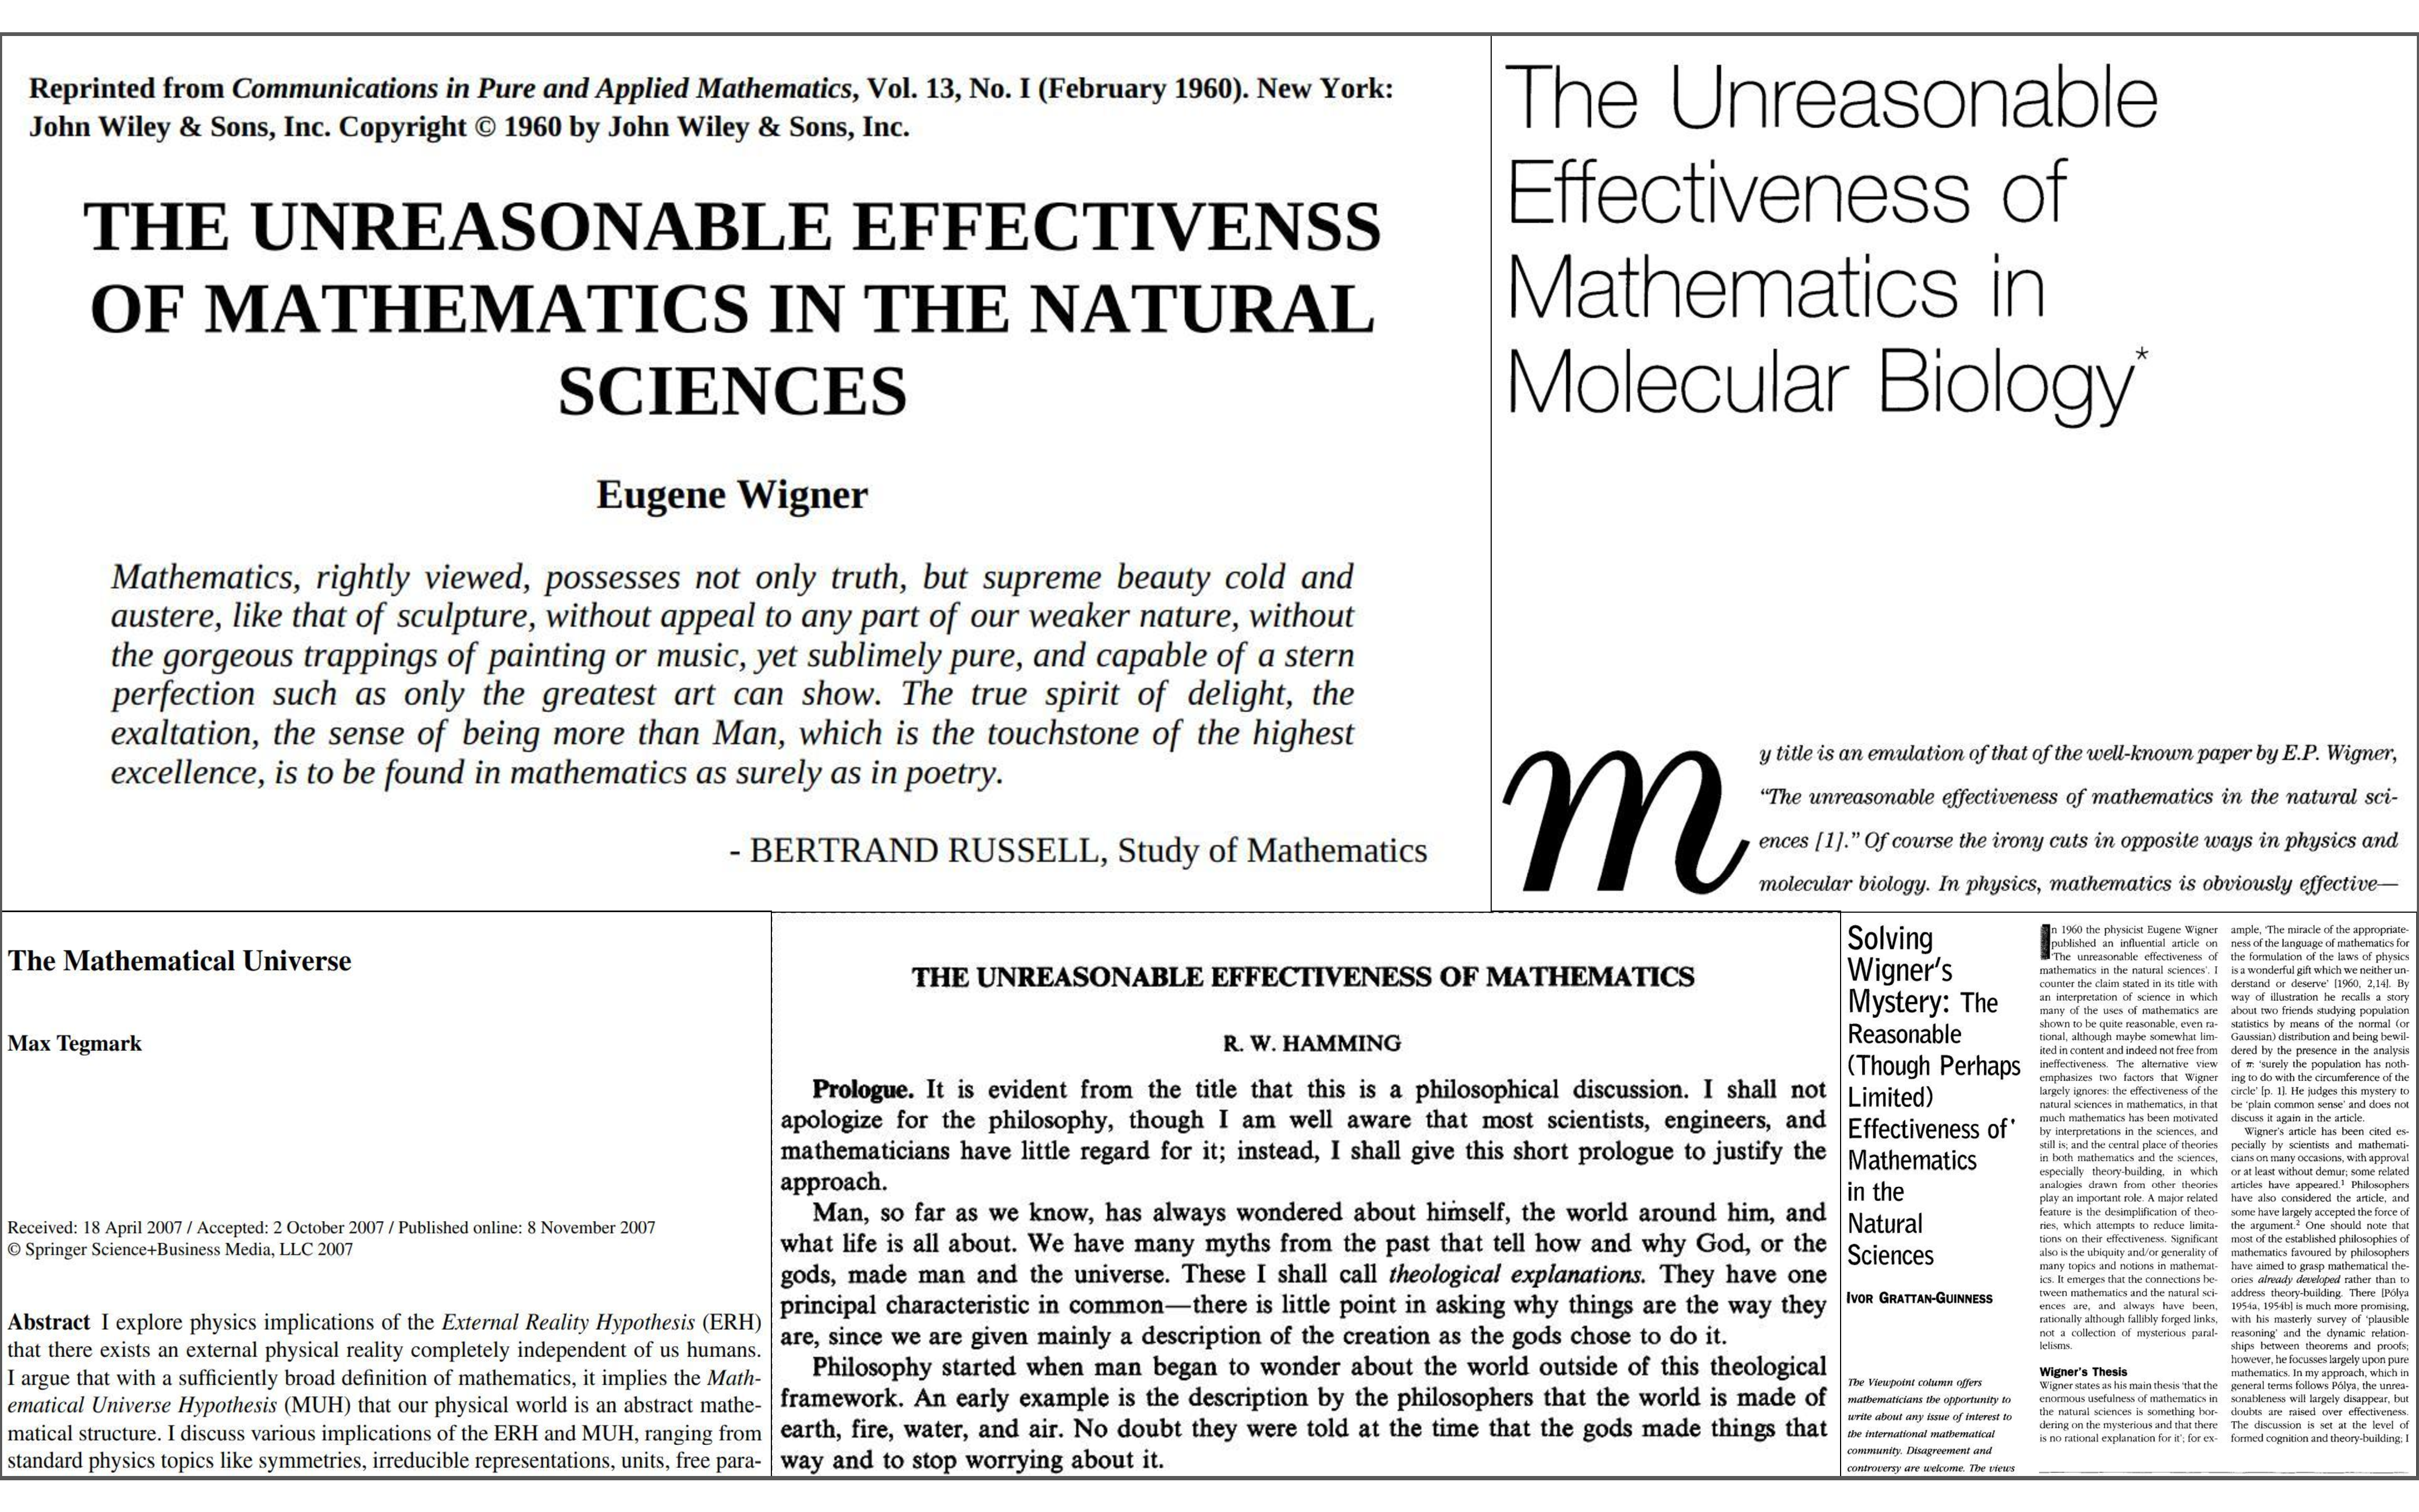
\includegraphics[width=1\linewidth]{images/EffectinvenessOFMath.pdf}
	\caption{A series of papers written after Wigner's famous article published in 1960 \cite{Wigner1995}. Several famous scientists of the time responded to this paper, by expanding the ideas to particular fields, among which are \cite{Hamming1980},  \cite{Lesk2000},  \cite{Tegmark2008}, and \cite{GrattanGuinness2008}. }
	\label{fig:mathmodelingmatheffectiveness}
\end{figure}

\FloatBarrier

\section{STEP II: Mathematical Analysis of the Model in Hand}
After doing the STEP I appropriately, we will have a mathematical description of the phenomena in our hand. This mathematical formulation on the problem can come in my different flavors and forms, We can categorize them by considering their different aspects, like being a discrete or continuous model, being a deterministic or stochastic model, etc. Each of these formulations will have its own appropriate way of treating. So I will discuss their subsequence steps separately.
 
 
\subsection{STEP II: PDE models}
After converting the natural phenomena to a mathematical model containing PDEs, we will have a domain, and a PDE. For instance, let $ \Omega \subset \R^2 $, and we define
\begin{align*}
	-\Delta u  &= g, \qquad \text{on }\Omega, \\
	u &= 0, \qquad \text{on } \partial \Omega.
\end{align*}
In this particular problem, we have a domain, on which we are interested in finding a mapping $ u:\Omega \to \R $ whose partial derivatives satisfies a certain equation. Our first goal is to determine if this problem has a solution (existence), and then to see if the problem as a unique solution (uniqueness), and then to see if the solution is stable (i.e. bounded by the given data). 

\begin{summary}
	Given a PDE in hand, it is important to see if the problem is well-posed (in the sense  of Hadamard). I.e.
	\begin{itemize}[noitemsep]
		\item a solution exists,
		\item the solution is unique, and
		\item the solution is stable.
		
	\end{itemize}
\end{summary}

\subsubsection{Different Formulations of the Problem: Strong vs. Weak Formulation}
To find the answers to these questions, we can formulate our problem in different ways, i.e. strong formulation, or a weak formulation. 